
\documentclass[8pt]{article}
\usepackage[utf8]{inputenc}
\usepackage{geometry}
\usepackage{xcolor}
\usepackage{titlesec}
\usepackage{fancyhdr}
\usepackage{tabularx}
\usepackage{array}
\usepackage{colortbl}
\usepackage{graphicx}
\usepackage{subcaption}
\usepackage{hyperref}
\usepackage{float}
\usepackage{ragged2e}
\usepackage{draftwatermark}
\usepackage{setspace}
\usepackage{tikz}
\SetWatermarkText{ Draft }
\SetWatermarkScale{1}

% Define colors
\definecolor{red}{HTML}{BE0D3E}
\definecolor{blue}{HTML}{004767}
\definecolor{darkblue}{HTML}{002F6C}
\definecolor{lightblue}{HTML}{E6F2F8}
\definecolor{darkgreen}{HTML}{1B5E20}
\definecolor{darkorange}{HTML}{FF6F00}
\definecolor{yellow}{HTML}{FDD835}
\definecolor{brown}{HTML}{6D4C41}
\definecolor{purple}{HTML}{7E57C2}
\definecolor{teal}{HTML}{26A69A}
\definecolor{brighterred}{HTML}{D32F2F}
\definecolor{brighterblue}{HTML}{0277BD}
\definecolor{brightergreen}{HTML}{388E3C}
\definecolor{brighterorange}{HTML}{FFA000}
\definecolor{brighteryellow}{HTML}{FBC02D}
\definecolor{darkerbrown}{HTML}{5D4037}
\definecolor{lightgrey}{HTML}{F4F4F4}
\definecolor{grey}{HTML}{BDBDBD}


% Page geometry
\geometry{left=1.7cm, right=0.8cm, top=1in, bottom=2in}
\pagestyle{fancy}
\fancyhf{}
\fancyhead[L]{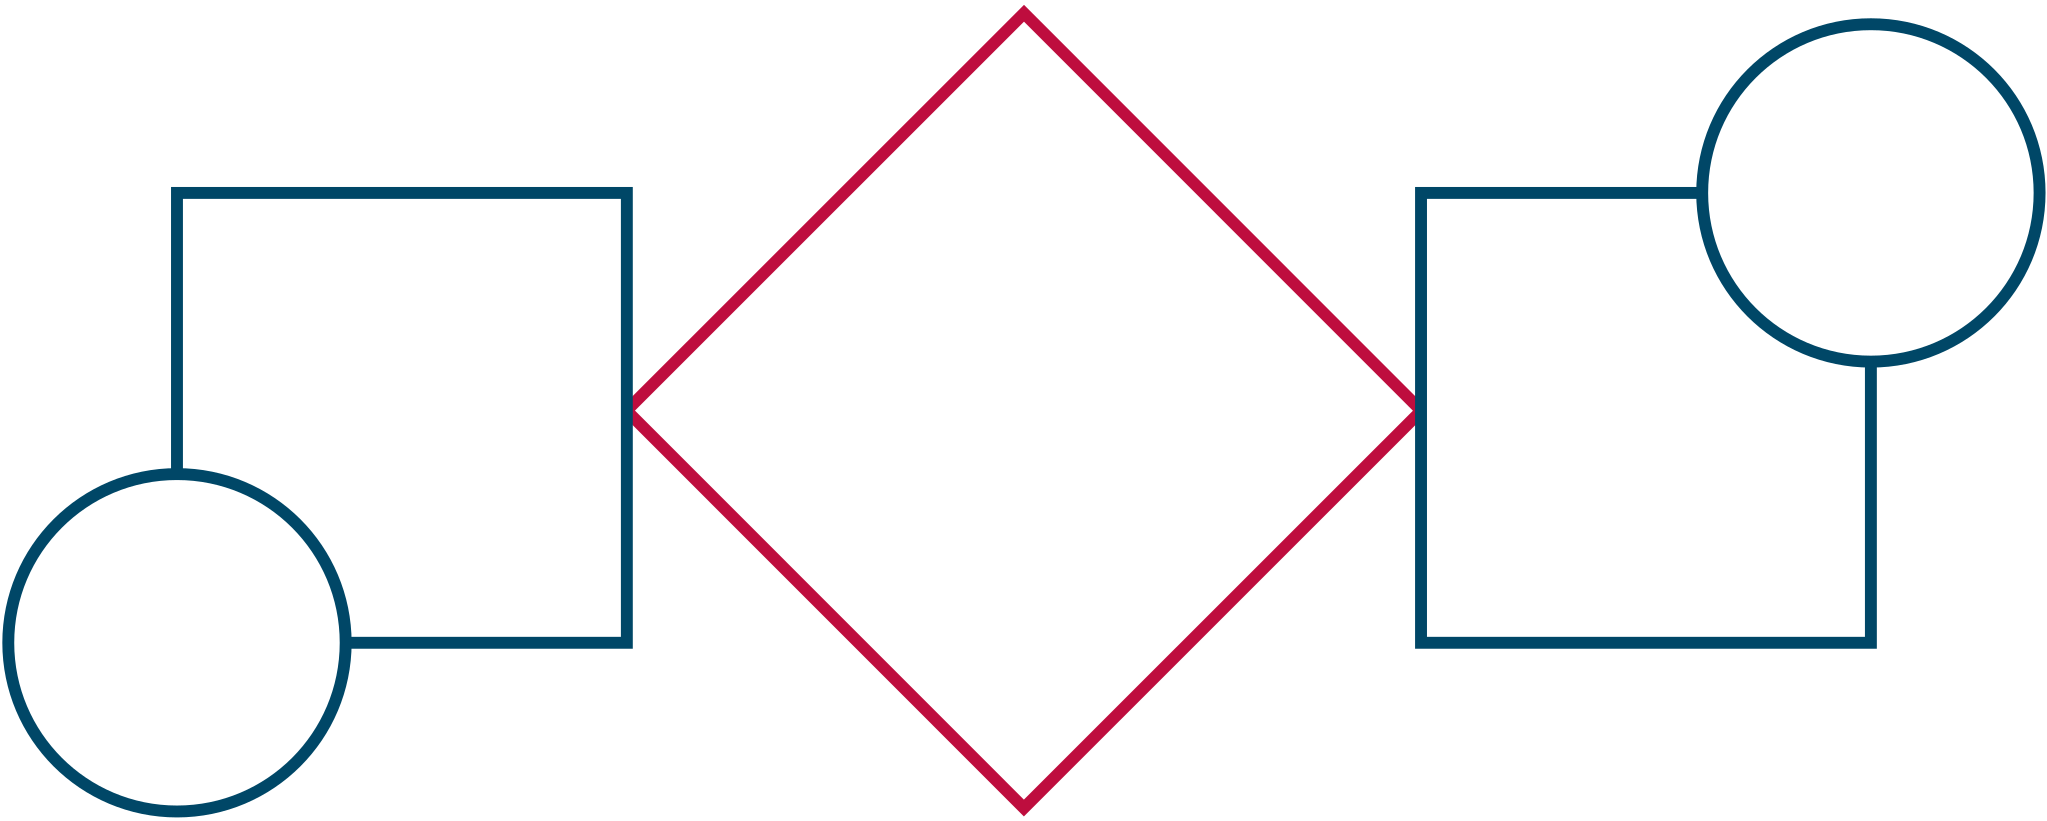
\includegraphics[height=1cm]{ /montrek/montrek/../static/logos/montrek_logo_variant.png  } }
\fancyhead[C]{\color{blue}\large\textbf{ Projekt Plan (Stand 23.01.2025) (Entwurf) }}
\fancyfoot[R]{\color{blue}\thepage}
\fancyfoot[L]{\color{grey}\footnotesize montrek UG (haftungsbeschränkt)\newline Taunusstrasse 25\newline 65183 Wiesbaden, DE\newline Registergericht: Amtsgericht Wiesbaden\newline USt-IdNr.: DE 367 918 366\newline Unternehmensführung: Vincent Mohiuddin, Dr. Christoph Hombach }
\renewcommand{\headrulewidth}{2pt}
\renewcommand{\headrule}{\hbox to\headwidth{\color{blue}\leaders\hrule height \headrulewidth\hfill}}
\setlength{\headsep}{1in}
\renewcommand{\footrulewidth}{1pt}
\setstretch{0.9}

% Fonts and colors
\usepackage{fontspec}
\setmainfont{Arial}

% Title formats
\titleformat*{\section}{\large\bfseries\color{blue}}
\titleformat*{\subsection}{\bfseries\color{blue}}

% Table settings
\renewcommand{\arraystretch}{1.2}

% Progress bars
\newcommand{\progressbar}[2]{
    % #1: Width percentage (0-100)
    % #2: Label (e.g., percentage)
    \begin{tikzpicture}
        \draw[fill=brightergreen, draw=none] (0, 0) rectangle (#1*0.01*\linewidth, 0.3);
        \draw[draw=black] (0, 0) rectangle (\linewidth, 0.3);
        \node[anchor=center] at (0.5*\linewidth, 0.15) {\color{blue}\textbf{#2}};
    \end{tikzpicture}
}

% Captions
\DeclareCaptionFormat{custom}
{%
  \textbf{\color{blue} \large #3}
}
\captionsetup{format=custom}
\begin{document}


\subsection*{Projekt Datenbank und Externalitätenmodel}

\begin{table}[H]
\begin{tabular}{ >{\raggedright\arraybackslash}p{ 0.49000\textwidth}>{\raggedleft\arraybackslash}p{ 0.49000\textwidth} }
\begin{minipage}[t]{0.49\textwidth}
\begin{table}[H]
\centering
\small
\arrayrulecolor{lightgrey}
\setlength{\tabcolsep}{2pt}
\renewcommand{\arraystretch}{1.0}
\caption{}
\begin{tabularx}{\textwidth}{|X|X|}
\hline
\cellcolor{blue}\color{white}\textbf{Name} &  \color{black} Datenbank und Externalitätenmodel \\
\hline
\cellcolor{blue}\color{white}\textbf{Projektstart} &\cellcolor{lightblue}  \color{black} 2024-07-04 \\
\hline
\cellcolor{blue}\color{white}\textbf{Projektende} &  \color{black} 2024-09-06 \\
\hline
\end{tabularx}
\end{table}
\end{minipage}
\begin{minipage}[t]{0.49\textwidth}
\begin{table}[H]
\centering
\small
\arrayrulecolor{lightgrey}
\setlength{\tabcolsep}{2pt}
\renewcommand{\arraystretch}{1.0}
\caption{}
\begin{tabularx}{\textwidth}{|X|X|}
\hline
\cellcolor{blue}\color{white}\textbf{Projektstatus} &  \color{black} COMPLETED \\
\hline
\cellcolor{blue}\color{white}\textbf{Kunde} &\cellcolor{lightblue}  \color{black} Effctl Capital GmbH \\
\hline
\end{tabularx}
\end{table}
\end{minipage}
 & \begin{justify}\textbf{Projektbeschreibung}\newline Aufstellen einer Datenbank, die Company, Bond, Equity und Marktdaten erfasst, sowie Externalitätenpreise und Externalitätenbewertungen von Unternehmen und Portfolios Datenimportprozess, der das Einlesen der Daten aus verschiedenen Quellen, Merging- und Cleaningprozesse behinhaltet, sowie eine Historisierung der Prozesse darstellt Die Logik zur Berechnung der Externalitätenbewertung von Unternehmen und das Speichern der Ergebnisse Das Reporten der Ergebnisse bezogen auf Equity und Bond Positionen von Unternehmen, die Teil eines Portfolios sind\end{justify} \\

\end{tabular}
\end{table}

\vspace{10mm}\begin{justify}\end{justify}\vspace{10mm}\subsection*{Arbeitspakete Übersicht}
\begin{table}[H]
\centering
\small
\arrayrulecolor{lightgrey}
\setlength{\tabcolsep}{1pt}
\renewcommand{\arraystretch}{0.5}
\caption{}
\begin{tabularx}{\textwidth}{|X|X|X|X|X|X|}
\hline
\rowcolor{blue}\color{white}\textbf{Name} & \color{white}\textbf{Description} & \color{white}\textbf{Start Date} & \color{white}\textbf{End Date} & \color{white}\textbf{Total Workdays} & \color{white}\textbf{Workdays Percentage} \\
\hline
\rowcolor{lightblue} \color{black} IO Setup & \color{black} Aufsetzen der Company DB Struktur, Import Mechanismen & \color{black} 2024-07-04 & \color{black} 2024-07-12 &\color{darkblue} 4.000 & \color{black} -\\
\hline
 \color{black} Merging und Cleaning & \color{black} Funktionalität zum Zusammenführen und Bereiningen der importierten Daten & \color{black} 2024-07-18 & \color{black} 2024-07-26 &\color{darkblue} 4.000 & \color{black} -\\
\hline
\rowcolor{lightblue} \color{black} Externality Valuation & \color{black} Aufsetzen der Externalitäten DB Struktur und Model Berechnungen & \color{black} 2024-08-01 & \color{black} 2024-08-09 &\color{darkblue} 4.000 &\progressbar{ 100.0 }{ 100.0\% }\\
\hline
\end{tabularx}
\end{table}

\subsection*{Arbeitspaket: IO Setup}

\begin{table}[H]
\begin{tabular}{ >{\raggedright\arraybackslash}p{ 0.49000\textwidth}>{\raggedleft\arraybackslash}p{ 0.49000\textwidth} }
\begin{minipage}[t]{0.49\textwidth}
\begin{table}[H]
\centering
\small
\arrayrulecolor{lightgrey}
\setlength{\tabcolsep}{2pt}
\renewcommand{\arraystretch}{1.0}
\caption{}
\begin{tabularx}{\textwidth}{|X|X|}
\hline
\cellcolor{blue}\color{white}\textbf{Name} &  \color{black} IO Setup \\
\hline
\cellcolor{blue}\color{white}\textbf{Startdatum} &\cellcolor{lightblue}  \color{black} 2024-07-04 \\
\hline
\cellcolor{blue}\color{white}\textbf{Enddatum} &  \color{black} 2024-07-12 \\
\hline
\end{tabularx}
\end{table}
\end{minipage}
\begin{minipage}[t]{0.49\textwidth}
\begin{table}[H]
\centering
\small
\arrayrulecolor{lightgrey}
\setlength{\tabcolsep}{2pt}
\renewcommand{\arraystretch}{1.0}
\caption{}
\begin{tabularx}{\textwidth}{|X|X|}
\hline
\cellcolor{blue}\color{white}\textbf{Total Workdays} & \color{darkblue} 4.000 \\
\hline
\cellcolor{blue}\color{white}\textbf{Workdays Percentage} &\cellcolor{lightblue}  \color{black} - \\
\hline
\end{tabularx}
\end{table}
\end{minipage}
 & \begin{justify}\textbf{Beschreibung}\newline Aufsetzen der Company DB Struktur, Import Mechanismen\end{justify} \\

\end{tabular}
\end{table}

\vspace{10mm}
\begin{table}[H]
\centering
\small
\arrayrulecolor{lightgrey}
\setlength{\tabcolsep}{1pt}
\renewcommand{\arraystretch}{0.5}
\caption{}
\begin{tabularx}{\textwidth}{|X|X|X|X|X|}
\hline
\rowcolor{blue}\color{white}\textbf{Item Name} & \color{white}\textbf{Item Status} & \color{white}\textbf{Item Description} & \color{white}\textbf{Workblock} & \color{white}\textbf{No Of Days} \\
\hline
\rowcolor{lightblue} \color{black} IO Setup & \color{black} PREPARATION & \color{black} Aufsetzen der Company DB Struktur, Import Mechanismen & \color{black} 4 Days Block &\color{darkblue} 4.000\\
\hline
\end{tabularx}
\end{table}

\subsection*{Arbeitspaket: Merging und Cleaning}

\begin{table}[H]
\begin{tabular}{ >{\raggedright\arraybackslash}p{ 0.49000\textwidth}>{\raggedleft\arraybackslash}p{ 0.49000\textwidth} }
\begin{minipage}[t]{0.49\textwidth}
\begin{table}[H]
\centering
\small
\arrayrulecolor{lightgrey}
\setlength{\tabcolsep}{2pt}
\renewcommand{\arraystretch}{1.0}
\caption{}
\begin{tabularx}{\textwidth}{|X|X|}
\hline
\cellcolor{blue}\color{white}\textbf{Name} &  \color{black} Merging und Cleaning \\
\hline
\cellcolor{blue}\color{white}\textbf{Startdatum} &\cellcolor{lightblue}  \color{black} 2024-07-18 \\
\hline
\cellcolor{blue}\color{white}\textbf{Enddatum} &  \color{black} 2024-07-26 \\
\hline
\end{tabularx}
\end{table}
\end{minipage}
\begin{minipage}[t]{0.49\textwidth}
\begin{table}[H]
\centering
\small
\arrayrulecolor{lightgrey}
\setlength{\tabcolsep}{2pt}
\renewcommand{\arraystretch}{1.0}
\caption{}
\begin{tabularx}{\textwidth}{|X|X|}
\hline
\cellcolor{blue}\color{white}\textbf{Total Workdays} & \color{darkblue} 4.000 \\
\hline
\cellcolor{blue}\color{white}\textbf{Workdays Percentage} &\cellcolor{lightblue}  \color{black} - \\
\hline
\end{tabularx}
\end{table}
\end{minipage}
 & \begin{justify}\textbf{Beschreibung}\newline Funktionalität zum Zusammenführen und Bereiningen der importierten Daten\end{justify} \\

\end{tabular}
\end{table}

\vspace{10mm}
\begin{table}[H]
\centering
\small
\arrayrulecolor{lightgrey}
\setlength{\tabcolsep}{1pt}
\renewcommand{\arraystretch}{0.5}
\caption{}
\begin{tabularx}{\textwidth}{|X|X|X|X|X|}
\hline
\rowcolor{blue}\color{white}\textbf{Item Name} & \color{white}\textbf{Item Status} & \color{white}\textbf{Item Description} & \color{white}\textbf{Workblock} & \color{white}\textbf{No Of Days} \\
\hline
\rowcolor{lightblue} \color{black} Merging und Cleaning & \color{black} PREPARATION & \color{black} Funktionalität zum Zusammenführen und Bereiningen der importierten Daten & \color{black} 4 Days Block &\color{darkblue} 4.000\\
\hline
\end{tabularx}
\end{table}

\subsection*{Arbeitspaket: Externality Valuation}

\begin{table}[H]
\begin{tabular}{ >{\raggedright\arraybackslash}p{ 0.49000\textwidth}>{\raggedleft\arraybackslash}p{ 0.49000\textwidth} }
\begin{minipage}[t]{0.49\textwidth}
\begin{table}[H]
\centering
\small
\arrayrulecolor{lightgrey}
\setlength{\tabcolsep}{2pt}
\renewcommand{\arraystretch}{1.0}
\caption{}
\begin{tabularx}{\textwidth}{|X|X|}
\hline
\cellcolor{blue}\color{white}\textbf{Name} &  \color{black} Externality Valuation \\
\hline
\cellcolor{blue}\color{white}\textbf{Startdatum} &\cellcolor{lightblue}  \color{black} 2024-08-01 \\
\hline
\cellcolor{blue}\color{white}\textbf{Enddatum} &  \color{black} 2024-08-09 \\
\hline
\end{tabularx}
\end{table}
\end{minipage}
\begin{minipage}[t]{0.49\textwidth}
\begin{table}[H]
\centering
\small
\arrayrulecolor{lightgrey}
\setlength{\tabcolsep}{2pt}
\renewcommand{\arraystretch}{1.0}
\caption{}
\begin{tabularx}{\textwidth}{|X|X|}
\hline
\cellcolor{blue}\color{white}\textbf{Total Workdays} & \color{darkblue} 4.000 \\
\hline
\cellcolor{blue}\color{white}\textbf{Workdays Percentage} &\cellcolor{lightblue} \progressbar{ 100.0 }{ 100.0\% } \\
\hline
\end{tabularx}
\end{table}
\end{minipage}
 & \begin{justify}\textbf{Beschreibung}\newline Aufsetzen der Externalitäten DB Struktur und Model Berechnungen\end{justify} \\

\end{tabular}
\end{table}

\vspace{10mm}
\begin{table}[H]
\centering
\small
\arrayrulecolor{lightgrey}
\setlength{\tabcolsep}{1pt}
\renewcommand{\arraystretch}{0.5}
\caption{}
\begin{tabularx}{\textwidth}{|X|X|X|X|X|}
\hline
\rowcolor{blue}\color{white}\textbf{Item Name} & \color{white}\textbf{Item Status} & \color{white}\textbf{Item Description} & \color{white}\textbf{Workblock} & \color{white}\textbf{No Of Days} \\
\hline
\rowcolor{lightblue} \color{black} Externality Valuation & \color{black} COMPLETED & \color{black} Aufsetzen der Externalitäten DB Struktur und Model Berechnungen & \color{black} 4 Days Block &\color{darkblue} 4.000\\
\hline
\end{tabularx}
\end{table}



\end{document}

